\section{Review of Considered Optimization Methods}
\subsubsection{Hyperparameters control in AGS}

The parameter $r$ from (\ref{eq:step2}) affects the global convergence of AGS directly (see
\cite{strSergGO}, Chapter 8):
at high enough value of $r$, the method converges to all global minima of the objective function with
guarantee.
At the same time, according to (\ref{eq:step3_2}) and (\ref{step5}), at the infinitely high value of $r$, AGS turns into
the brute force search method on a uniform grid.

In the ideal case, in order to provide the highest convergence speed, the estimate of the Lipschitz
constant from (\ref{eq:step2})
should not be too overestimated, but in practice the actual value of $L$ from (\ref{eq:lip}) in
unknown, and one has either to take an obviously overestimated value of $r$ or to execute several
runs of AGS with different parameters. In order to resolve the problem of choosing $r$ to some extent,
let us use the following scheme:
\begin{itemize}
  \item execute $q$ iterations of AGS with $r=r_{max}$;
  \item execute $q$ iterations of AGS with $r=r_{min}$;
  \item repeat the above steps either until convergence or until the allowed number of iterations are
exhausted.
\end{itemize}

In the above algorithm, $r_{min} < r_{max}$, $q > 1$. Instead one parameter $r$, now
3 ones should be selected. However, according to the results of the numerical experiments, it is easier
than to find the optimal value of $r$.
Intuitively, the practical efficiency of the proposed scheme can be explained by the fact that now the
operation of the method takes place in two modes: the global search with $r=r_{max}$ and the local
one with $r=r_{min}$. If during the global search phase, the method approached the global minimum
whereas during the next phase, the estimate of the global minimum  would be refined rapidly.
If two phases are not enough, the process is continued. This way, a better trade-off
between the exploration and the exploitation is achieved.
Further, we will denote the method utilizing the scheme described above as AGS-AR.

\subsection{Other Optimization Methods}
\begin{itemize}
  \item \textbf{Multi Level Single Linkage} \cite{Kan1987StochasticGO}. MLSL is an improved
multistart algorithm.
  It samples low-discrepancy starting points and does local optimizations from them. In contrast to
the dummy multistart schemes
  MLSL uses some clustering heuristics to avoid multiple local descents to already explored local
minima.

  \item \textbf{DIRECT} \cite{Jones2009}. The algorithm is deterministic and recursively divides
the search space and forms a tree of hyper-rectangles (boxes). DIRECT uses the objective function
values and the Lipschitz condition (\ref{eq:lip}) to estimate promising boxes.

  \item \textbf{Locally-biased DIRECT (DIRECT$l$)} \cite{Gablonsky2001}. It's a variation of
DIRECT which pays less attention to non-promising boxes and therefore
  has less exploration power: it can converge faster on problems with few local minima, but lost the
global one in complicated cases.

  \item \textbf{Dual Simulated Annealing} \cite{XIANG1997216}. This stochastic method is a
combination of the Classical Simulated Annealing and the Fast Simulated Annealing coupled to a
strategy for applying a local search on accepted locations. It converges much faster than both parent
algorithms, CSA and FSA.

  \item \textbf{Differential Evolution} \cite{Storn1997}. DE is an adaptation of the original genetic
algorithm to
  the continuous search domain.

  \item \textbf{Controlled Random Search} \cite{Price1983}. The CRS starts with a set of random
points and then defines
  the next trial point in relation to a simplex chosen randomly from a stored configuration of points.
CRS in not an
  evolutional algorithm, although stores something like population and performs transformation
resembling a mutation.

  \item \textbf{StoGO} \cite{Madsen1998}. StoGO is dividing the search space into smaller hyper-
rectangles via a branch-and-bound approach,
  and searching them by a local-search algorithm, optionally including some randomness.

\end{itemize}

All the mentioned algorithms are available in source codes as parts of wide-spread optimization packages.
DIRECT, DIRECT$l$, CRS, MLSL and StoGO are part of the NLOpt library \cite{nlopt}.
Differential Evolution and DSA can be found in
the latest version of the SciPy \cite{scipy} package for Python.

\section{Tools for Comparison of Global Optimization Algorithms}

The use of the sets of test problems with known solutions generated by some random mechanisms is
one of commonly accepted approaches to comparing the optimization algorithms
\cite{Beiranvand2017}. In the present work, we will use two generators of test problems generating
the problems of different nature \cite{grishaginClass, Gaviano2003} \footnote{Software implementations of
these generators are available in source codes at the page \url{https://github.com/sovrasov/global-optimization-test-problems}}.

Let us denote the problem set obtained with the use of the first generator from \cite{grishaginClass}
as \(F_{GR}\). The mechanism of generation of the problems \(F_{GR}\) doesn't provide the
control of the problem complexity and of the number of local optima. However, the generated
functions are known to be the multiextremal ones essentially. Besides, the problems generated by
\(F_{GR}\) are the two-dimensional ones. In the present work, we will use 100 functions from the
class \(F_{GR}\) generated randomly.

The GKLS generator \cite{Gaviano2003} allows obtaining the problems of given dimensionality
with given number of extrema. Moreover, GKLS allows adjusting the complexity of the problems by
decreasing or increasing the size of the global minimum attractor. In
\cite{SergeyevKvasov2006} the parameters of the generator allowing generating the sets of 100
problems each of two levels of complexity (Simple and Hard) of the dimensionality equal to 2, 3, 4,
and 5 are given. Following the authors of the GKLS generator, we will use the parameters proposed
by them and, this way, add 800 more problems of various dimensionalities and complexity into the
test problem set.

Let us suppose a test problem to be solved if the optimization method executes the scheduled trial
\(y^k\) in a \(\delta\)-vicinity of the global minimum \(y^*\), i.e. $\left\|y^k-y^*\right\|\leq \delta
= \alpha\left\|b-a\right\|$, where \(a\) and \(b\) are the left and the right boundaries of the hypercube
from (\ref{eq:task}), $\alpha$ is relative precision. If this relation is not fulfilled before the expiration of the limit of the number of
trials, the problem was considered to be unsolved. The limit of the number of trials and $\alpha$ were set
for each problem class according to the dimensionality and complexity (see Table \ref{tab:limits}).

\begin{table}
\begin{center}
\caption{Trials limits and relative precision for the test problem classes}
  \begin{tabular}{|l|{c}|{c}|}
    \hline
  Problems class & Trials limit & $\alpha$\\
  \hline
  \(F_{GR}\) & 5000 & 0.01 \\
  \hline
  GKLS 2d Simple & 8000 & 0.01 \\
  \hline
  GKLS 2d Hard & 9000 & 0.01 \\
  \hline
  GKLS 3d Simple & 15000 & 0.01 \\
  \hline
  GKLS 3d Hard & 25000 & 0.01 \\
  \hline
  GKLS 4d Simple & 150000 & $\sqrt[4]{10^{-6}}$ \\
  \hline
  GKLS 4d Hard & 250000 & $\sqrt[4]{10^{-6}}$ \\
  \hline
  GKLS 5d Simple & 350000 & $\sqrt[5]{10^{-7}}$ \\
  \hline
  GKLS 5d Hard & 600000 & $\sqrt[5]{10^{-7}}$ \\
  \hline
  \end{tabular}
  \label{tab:limits}
\end{center}
\end{table}

Let us consider the averaged number of trials executed to solve a single problem and the number of
solved problems as the characteristics of the optimization method on each class. The less the number
of trials, the faster the method converges to a solution, hence the less times it turns to a potentially
computation-costly procedure of computing the objective function. The number of solved problems
evidences the reliability of the method at given parameters on the class of test problems being
solved. In order to make independent the quantities featuring the reliability and the speed of convergence,
averaged number of trials always was calculated taking into account solved problems only.

The average number of trials doesn't represent the real behavior of an optimization method
on a problems set in some cases. For an instance, if a method performs well on the most problems
and spends too much trials to solve the least several problems, we wouldn't catch such
case looking at the average number of trials only.
As an advanced measure of performance we will use the operating characteristic \cite{grishaginClass}.
It's defined by a set of points on the \((K, P)\) plane where \(K\) is the average number of search trials
conducted before satisfying the termination condition when minimizing a function
from a given class, and \(P\) is the proportion of problems solved successfully.
If at a given \(K\), the operating characteristic of a method goes higher than one
from another method, it means that at fixed search costs, the former method has a
greater probability of finding the solution. If some value of \(P\) is fixed, and the
characteristic of a method goes to the left from that of another method, the former
method requires fewer resources to achieve the same reliability.

\section{Results of Numerical Experiments}
\label{sec:experiments}
The results of various algorithms on different problem classes depend on the adjustments of
algorithms directly. In most cases, the authors of software implementations are oriented onto the
problems of medium difficulty. In order to obtain a satisfactory result when solving the essentially
multiextremal problems, a correction of some parameters is required. When conducting the
comparison, the following parameters for the methods were employed:
\begin{itemize}
  \item in the AGS-AR method, the parameter of alternation the
  global and local stages $q$ was set to be equal to $50\cdot\log_2(N-1)\cdot N^2$, also $r_{min}=3,\:r_{max}=2\cdot r_{min}$;
  \item in the DIRECT and DIRECT\(l\) methods, the parameter \(\epsilon=10^{-4}\);
  \item in the SDA method, the parameter \(visit=2.72\).
\end{itemize}

The rest parameters were varied subject to the problem class (see Table \ref{tab:params}).
For the AGS the value ot the $r$ parameter, such that the method solves all problems and performs the minimum amount of trials,
was estimated by brute force on the uniform grid with step $0.1$.

\begin{table}
\begin{center}
\caption{Class-specific parameters of the optimization algorithms}
  \begin{tabular}{|l|{c}|{c}|{c}|}
    \hline
    & AGS & CRS & DE\\
  \hline
  \(F_{GR}\) & \(r=3\) & popsize=150 & mutation=(1.1,1.9), popsize=60 \\
  \hline
  GKLS 2d Simple & \(r=4.6\) & popsize=200 & mutation=(1.1,1.9), popsize=60 \\
  \hline
  GKLS 2d Hard & \(r=6.5\) & popsize=400 & mutation=(1.1,1.9), popsize=60 \\
  \hline
  GKLS 3d Simple & \(r=3.7\) & popsize=1000 & mutation=(1.1,1.9), popsize=70 \\
  \hline
  GKLS 3d Hard & \(r=4.4\) & popsize=2000 & mutation=(1.1,1.9), popsize=80 \\
  \hline
  GKLS 4d Simple & \(r=4.7\) & popsize=8000 & mutation=(1.1,1.9), popsize=90 \\
  \hline
  GKLS 4d Hard & \(r=4.9\) & popsize=16000 & mutation=(1.1,1.9), popsize=100 \\
  \hline
  GKLS 5d Simple & \(r=4\) & popsize=25000 & mutation=(1.1,1.9), popsize=120 \\
  \hline
  GKLS 5d Hard & \(r=4\) & popsize=30000 & mutation=(1.1,1.9), popsize=140 \\
  \hline
\end{tabular}
  \label{tab:params}
\end{center}
\end{table}

\begin{table}
\begin{center}
\caption{Averaged number of trials executed by optimization methods for solving the test
optimization problems}
\resizebox{\textwidth}{!}{%
  \begin{tabular}{|l|{c}|{c}|{c}|{c}|{c}|{c}|{c}|{c}|{c}|{c}|}
    \hline
    & AGS & AGS-AR & CRS & DIRECT & DIRECT\(l\) & MLSL & SDA & DE & StoGO \\
  \hline
  \(F_{GR}\)     & 193.1 & 248.3 & 400.3 & \textbf{182.2} & 214.9 & 947.2 & 691.2 & 1257.3 & 1336.8 \\
  \hline
  GKLS 2d Simple & 254.9 & 221.6 & 510.6 & \textbf{189.0} & 255.2 & 556.8 & 356.3 & 952.2 & 1251.5 \\
  \hline
  GKLS 2d Hard   & \textbf{728.7} & 785.0 & 844.7 & 985.4 & 1126.7 & 1042.5 & 1637.9 & 1041.1 & 2532.2 \\
  \hline
  GKLS 3d Simple &  1372.1 & 1169.5 & 4145.8 & \textbf{973.6} & 1477.8 & 4609.2 & 2706.5 & 5956.9 & 3856.1 \\
  \hline
  GKLS 3d Hard   &  3636.1 & \textbf{1952.1} & 6787.0 & 2298.7 & 3553.3 & 5640.1 & 4708.4 & 6914.3 & 7843.2 \\
  \hline
  GKLS 4d Simple &  5729.8 & \textbf{4919.1} & 19883.6 & 7328.8 & 15010.0 & 41484.8 & 22066.0 & 6271.2 & 29359.2 \\
  \hline
  GKLS 4d Hard   &  13113.4 & \textbf{12860.1} & 27137.4 & 22884.4 & 55596.1 & 80220.1 & 68048.0 & 12487.6 & 58925.5  \\
  \hline
  GKLS 5d Simple &  \textbf{5821.5} & 6241.3 & 62921.7 & 5966.1 & 10795.5 & 52609.2 & 34208.8 & 20859.4 & 69206.8 \\
  \hline
  GKLS 5d Hard   &  \textbf{17008.6} & 21555.1 & 87563.9 & 61657.3 & 148637.8 & 138011.8 & 115634.6 & 26850.0 & 141886.5 \\
  \hline
\end{tabular}}
  \label{tab:trials}
\end{center}
\end{table}

The results of running the optimization methods on the considered problem classes are presented in
Tables \ref{tab:trials}, \ref{tab:solved}. The DIRECT, AGS and AGS-AR methods have demonstrated the
best convergence speed on all classes, at that AGS-AR inferior to DIRECT on the 2d problems from the
Simple classes and has an advantage on the problems of the Hard classes. As one can see from Table
\ref{tab:solved}, the deterministic methods (AGS, AGS-AR, DIRECT, and DIRECT\(l\)) were the
most reliable. Among the stochastic methods, MLSL and SDA have demonstrated the highest
reliability.

\begin{table}
\begin{center}
\caption{Number of test optimization problems solved by the methods}
  \begin{tabular}{|l|{c}|{c}|{c}|{c}|{c}|{c}|{c}|{c}|{c}|{c}|}
    \hline
    & AGS & AGS-AR & CRS & DIRECT & DIRECT\(l\) & MLSL & SDA & DE & StoGO \\
  \hline
  \(F_{GR}\)     &  100 & 100 & 76 & 100 & 100 & 97 & 96 & 96 & 67\\
  \hline
  GKLS 2d Simple &  100 & 100 & 85 & 100 & 100 & 100 & 100 & 98 & 90\\
  \hline
  GKLS 2d Hard   &  100 & 97 & 74 & 100 & 100 & 100 & 93 & 85 & 77 \\
  \hline
  GKLS 3d Simple &  100 & 100 & 75 & 100 & 100 & 100 & 89 & 86 & 44 \\
  \hline
  GKLS 3d Hard   &  100 & 100 & 72 & 100 & 99 & 100 & 88 & 77 & 43 \\
  \hline
  GKLS 4d Simple &  100 & 100 & 74 & 100 & 100 & 94 & 82 & 68 & 72 \\
  \hline
  GKLS 4d Hard   &  100 & 100 & 60 & 99 & 99 & 94 & 73 & 55 & 69  \\
  \hline
  GKLS 5d Simple &  100 & 100 & 86 & 100 & 100 & 98 & 100 & 88 & 82  \\
  \hline
  GKLS 5d Hard   &  100 & 100 & 77 & 100 & 93 & 79 & 86 & 77 & 78 \\
  \hline
  \end{tabular}
  \label{tab:solved}
\end{center}
\end{table}

\begin{figure}[ht]
  \centering
  \subfloat[4d Simple]{{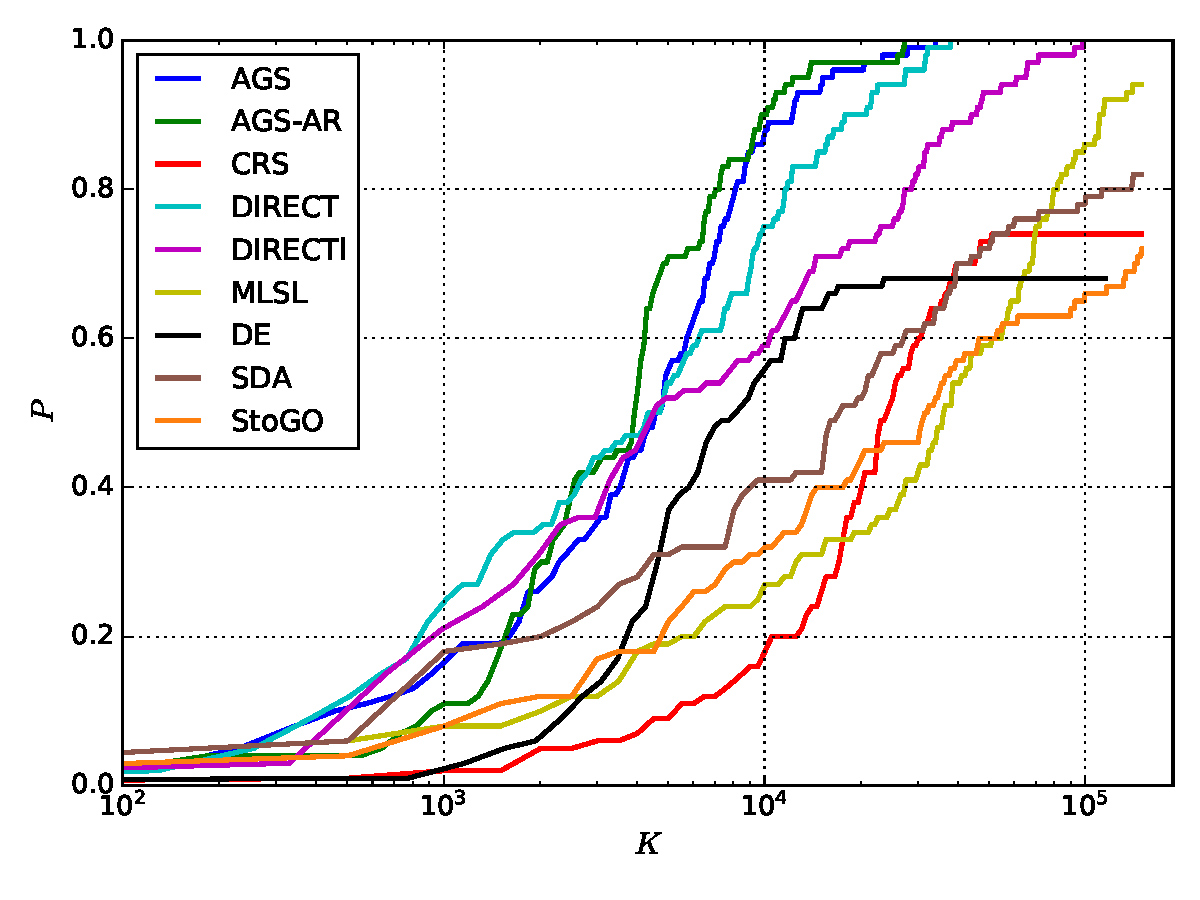
\includegraphics[width=.5\textwidth]{images/gklss4d.pdf}}\label{fig:s4d}}
  \subfloat[4d Hard]{{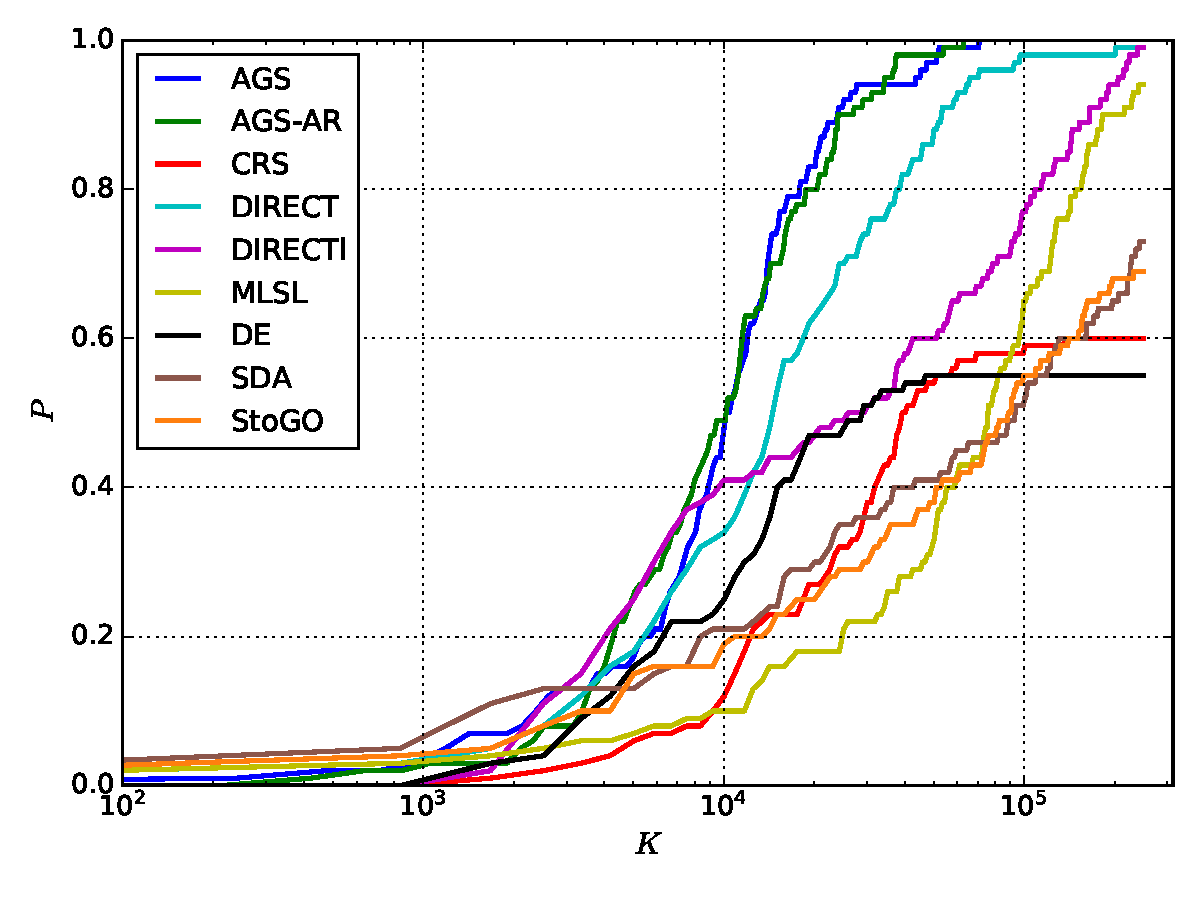
\includegraphics[width=.5\textwidth]{images/gklsh4d.pdf}}\label{fig:h4d}}

  \subfloat[5d Simple]{{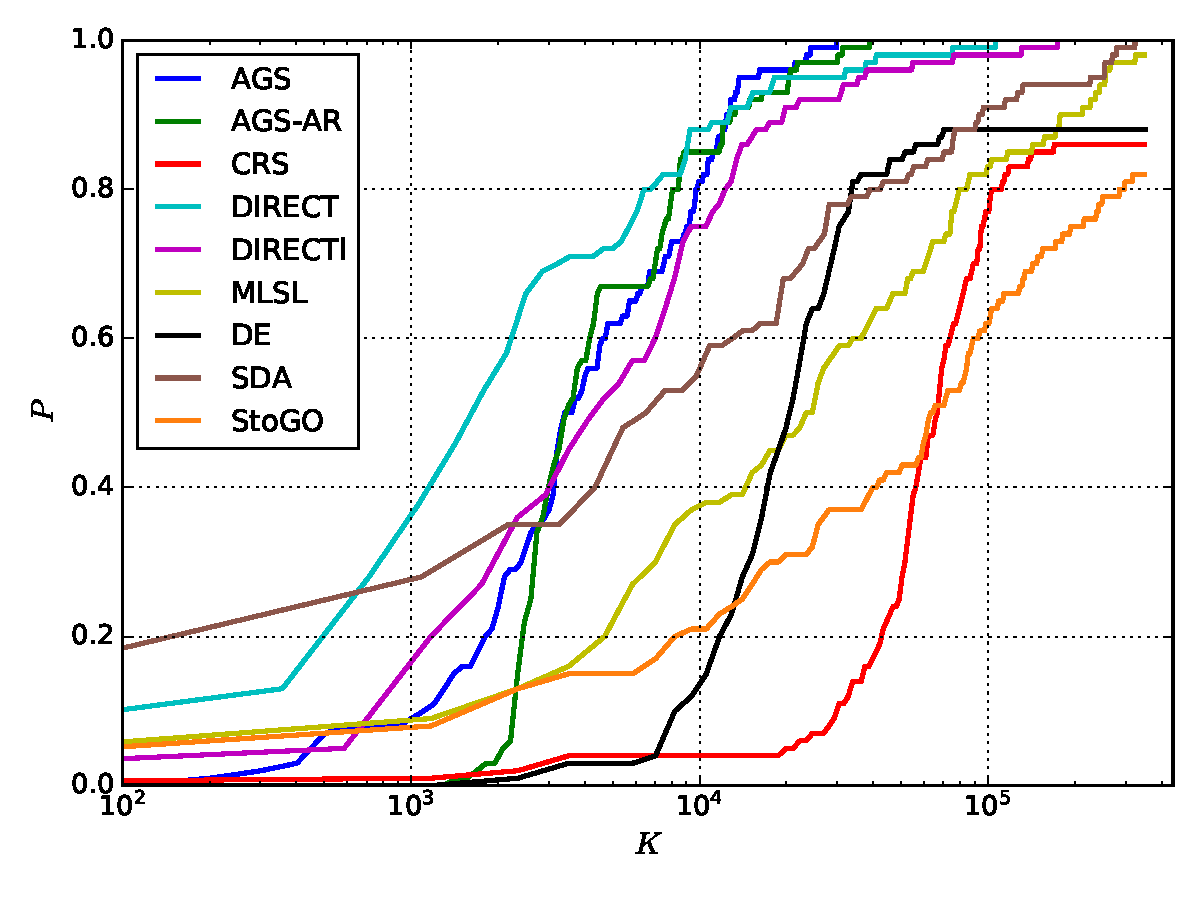
\includegraphics[width=.5\textwidth]{images/gklss5d.pdf}}\label{fig:s5d}}
  \subfloat[5d Hard]{{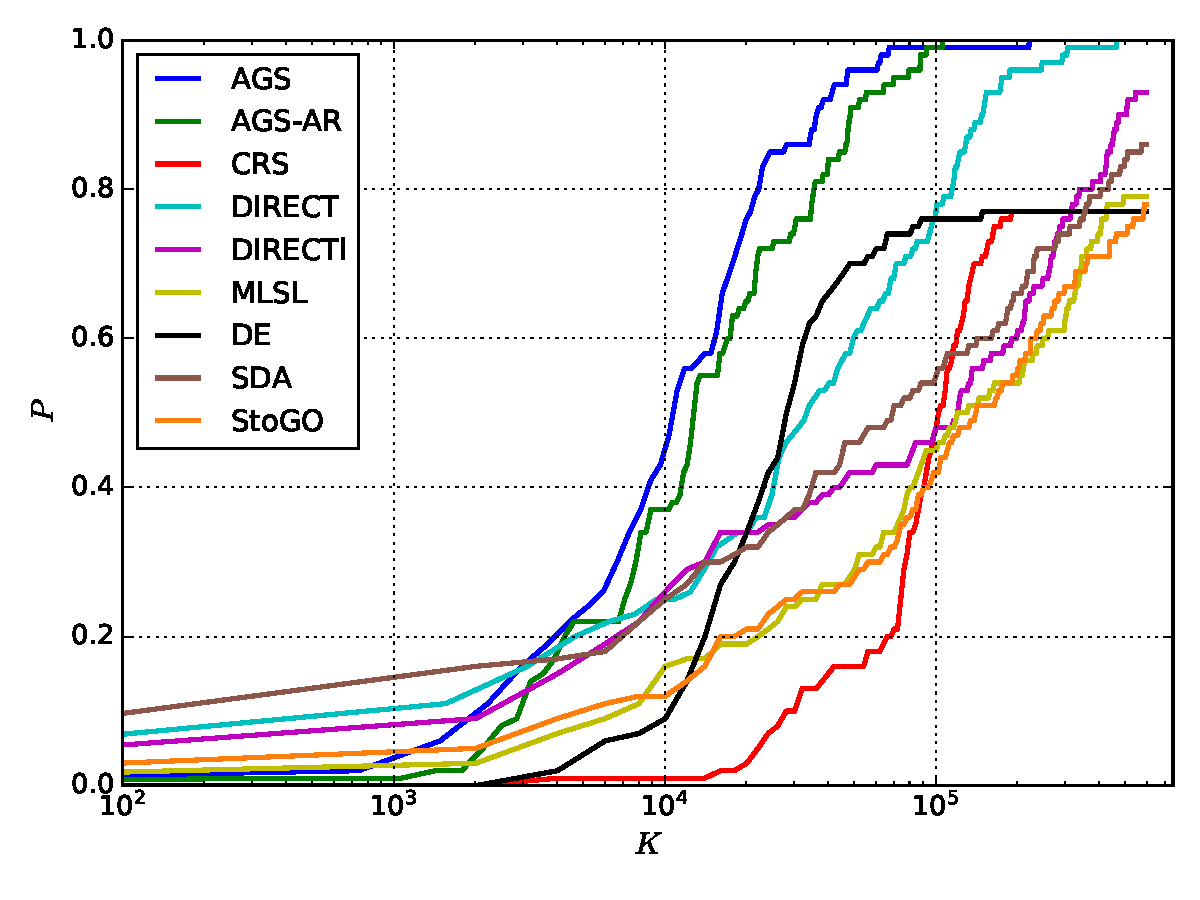
\includegraphics[width=.5\textwidth]{images/gklsh5d.pdf}}\label{fig:h5d}}
  \caption{Operating characteristics of the algorithms when solving problems from the GKLS 4d and 5d classes. Best viewed in color.}
\end{figure}

Operating characteristic of the methods (Figures \ref{fig:s4d}, \ref{fig:h4d}, \ref{fig:s5d}, \ref{fig:h5d})
demonstrates that AGS and AGS-AR faster than the other methods achieve 100\% success rate. Also on GKLS 5d Simple the DIRECT
generally has the best performance, but there are several hard problems that affect it's average number of
trials metric.

\paragraph{Robustness of AGS and AGS-AR to the Hyperparameters Choice.}

In order to investigate the influence of hyperparameters to the convergence speed of the AGS and AGS-AR,
experiments with the following settings were conducted on the problems from GKLS 5d Simple class:
\begin{itemize}
  \item AGS with $r=4$ (like in the Table \ref{tab:params});
  \item AGS with $r=6$;
  \item AGS-AR with parameters from the beginning of the Section \ref{sec:experiments}
  ($q=50\cdot\log_2(4)\cdot 25 = 2500$, $r_{min}=3,\:r_{max}=2\cdot r_{min}$);
  \item AGS-AR with $r_{max}=8$ and other parameters from the previous experiment;
  \item AGS-AR with $q=1000$ and other parameters from the beginning of the Section \ref{sec:experiments};
\end{itemize}

\begin{figure}[ht]
  \centering
  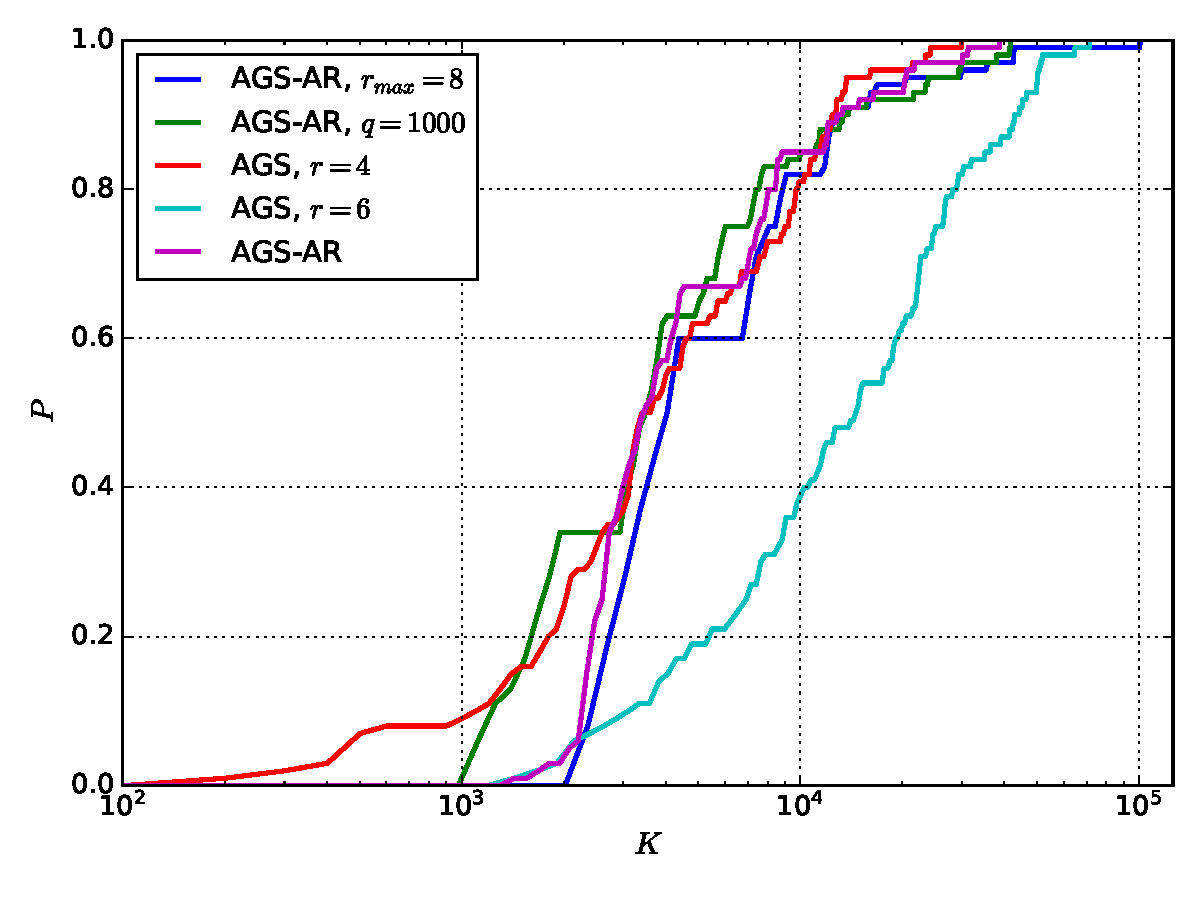
\includegraphics[width=.6\textwidth]{images/ar_stab.pdf}
  \caption{Operating characteristics of AGS and AGS-AR with different hyperparameters
  when solving problems from the GKLS 5d Simple classe. Best viewed in color.}
  \label{fig:stability}
\end{figure}

The operating characteristics collected in the experiments described above are shown in the Figure \ref{fig:stability}.
AGS with $r=6$ (the cyan-colored curve) shows the worst convergence speed, which indicates that AGS is very sensitive to choice of $r$.
Since on the start AGS-AR has the same value of $r$ as AGS with $r=6$, operating characteristics of these methods
are identical up to $K=2500$. After that point AGS-AR switches to $r=3$ and rapidly begins to increase the amount of solved problems
until the next exploration phase on $K=5000$. Intervals where AGS-AR works with $r=r_{max}$ are visible on the operating characteristics as plateaus.
Variations of $r$ and $q$ didn't drastically change the operating characteristic of AGS-AR. The latter observation shows robustness of the proposed
AGS modification with the alternating parameter $r$.

\section{Conclusions}

In the present paper, several global optimization algorithms were considered.
A comparison of efficiencies of these ones has been done on a set of test problems.
Also a scheme of hyperparameters control for the AGS algorithms was proposed and evaluated.
The results presented in this work allow making the following conclusions:
\begin{itemize}
  \item the proposed modification of the stock AGS, AGS-AR allows to pay less attention to initial hyperparameter tuning and
  performs on-par with properly tuned AGS;
  \item AGS-AR method has demonstrated the convergence
  speed and reliability at the level of DIRECT and exceeds many other algorithms, the open-source
  implementations of which are available;
  \item the stochastic optimization methods inferior to the deterministic ones in the convergence
speed and in reliability. It is manifested especially strongly on more complex multiextremal
problems.
\end{itemize}
